
This enables us, in our tests to merely require that an interface (a client of it, that is) is provided to use, rather than having to explicitly elaborate the code in the test case.

\begin{figure}
 \centering
 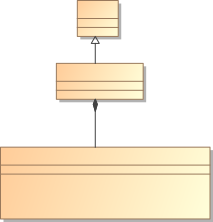
\includegraphics[scale=0.60]{img/support-tools-recepionist-example}
 \caption{support-tools-recepionist-example}
 \label{fig:support-tools-recepionist-example}
\end{figure}

%\begin{figure}
% \centering
%\missingfigure[figwidth=6cm]{This is some text that is with the todo and in the figure}
% \caption{support-tools-recepionist-example}
% \label{fig:support-tools-recepionist-example}
%\end{figure}